\chapter{提案手法}
本研究ではレスキュー犬行動推定のために,動画像・音声のマルチラベル分類を行う.
そのため,レスキュー犬訓練データセットを認識するための手法を提案する.

入力を動画とした際に,動画から静止画像と音声を切り出し,optical flow画像を生成する.
この3つをそれぞれ別のストリームに入力し,それぞれの出力を元にレスキュー犬の行動を推定する.概念図を~\ref{easy_image}に示す.
\begin{figure}[H]
 \begin{center}
  \includegraphics[width=10cm]{./Figures/easy_image.eps}
  \caption{提案手法の概要.入力動画から複数データを抽出し,それぞれ別のストリームへ入力する.各ストリームの出力をもとに,動画のレスキュー犬行動推定結果を最終出力とする.}
  \label{easy_image}
 \end{center}
\end{figure}

\section{音声と画像を用いたsound/image-based two-stream CNN}
1つ目の提案手法として,音声を用いたtwo-stream networkを提案する.
既存のtwo-stream networkを改造し,静止画と音声からの動画分類の手法である.
Two-stream networkと違い音声を用いるため,これをsound/image-based two-stream networkと呼称する.
sound/image-based two-stream networkのアーキテクチャを図~\ref{sound-two-stream}に示す.
これは画像ストリームと音声ストリームからなり,音声ストリームには音声から抽出したmfcc特徴を入力する.
画像ストリームには(3, 224, 224)次元の画像を入力とする.それぞれのストリームの出力を結合し,全結合層を通して各クラス毎の推定結果を得る.

本研究ではこのネットワークを一般的なシングルクラス分類ではなくマルチクラス推定に用いる.
まず入力となる動画から静止画像のフレーム($F_t$)を取り出し,直後の$F_{t+1}$間とのoptical flow画像($O_t$)を生成する.次に両画像から同じ構造の2つのネットワークを用いて特徴量の抽出を行う.
そして対応する音声($A_t$)からメル周波数ケプストラム係数($M_t$)を求め,前述とは異なる構造のネットワークを用いて($M_t$)から特徴量の抽出を行う.
最後にこれら2つあるいは3つの特徴量の組み合わせ毎に結合し,分類ネットワークでクラス分類を行う.
この際に,音声をフレームと同じサイズで切り出すと特徴が著しく失われるため入力音声には$F_t$の前後0.5秒ずつを用いた.動画あるいは音声から実際に犬の行動を推定する場合を想定し,現実的で取り扱いやすい時間としてこれを設定した.
分類はフレーム毎に行った.

シングルクラス分類の損失関数にはCrossEntropyLossを用いてクラス確率を求めたが,マルチクラス推定にはクラス毎にSoftMarginLossを用いた.
入力を$x$,出力を$y$,クラス数を$C$とすると,マルチクラス推定の損失関数SoftMarginLossは式~\ref{softmargin}に定義される.
推定クラスが正解なら$\Sigma$内の第2項,不正解なら第1項が計算に利用するように設計されており,推定ラベルによって関数が変わる.
本研究では11クラスあり,出力yは11次元のバイナリとする.
閾値=0.5とし,閾値以上のクラスを推定クラスとした.
\begin{equation}
\label{softmargin}
loss(x, y) = -\frac{1}{C} * \Sigma_{i} y[i] * log((1+exp(-x[i]))^{-1}) + (1 - y[i]) * log(\frac{exp(-x[i])}{1+exp(-x[i])})
\end{equation}

学習は全てにおいて100エポック行った.学習率は1e-03〜1e-06,バッチサイズは32〜128の範囲で学習毎に変え制限の中で最も良い精度の結果を評価した.


\begin{figure}[htbp]
 \begin{center}
  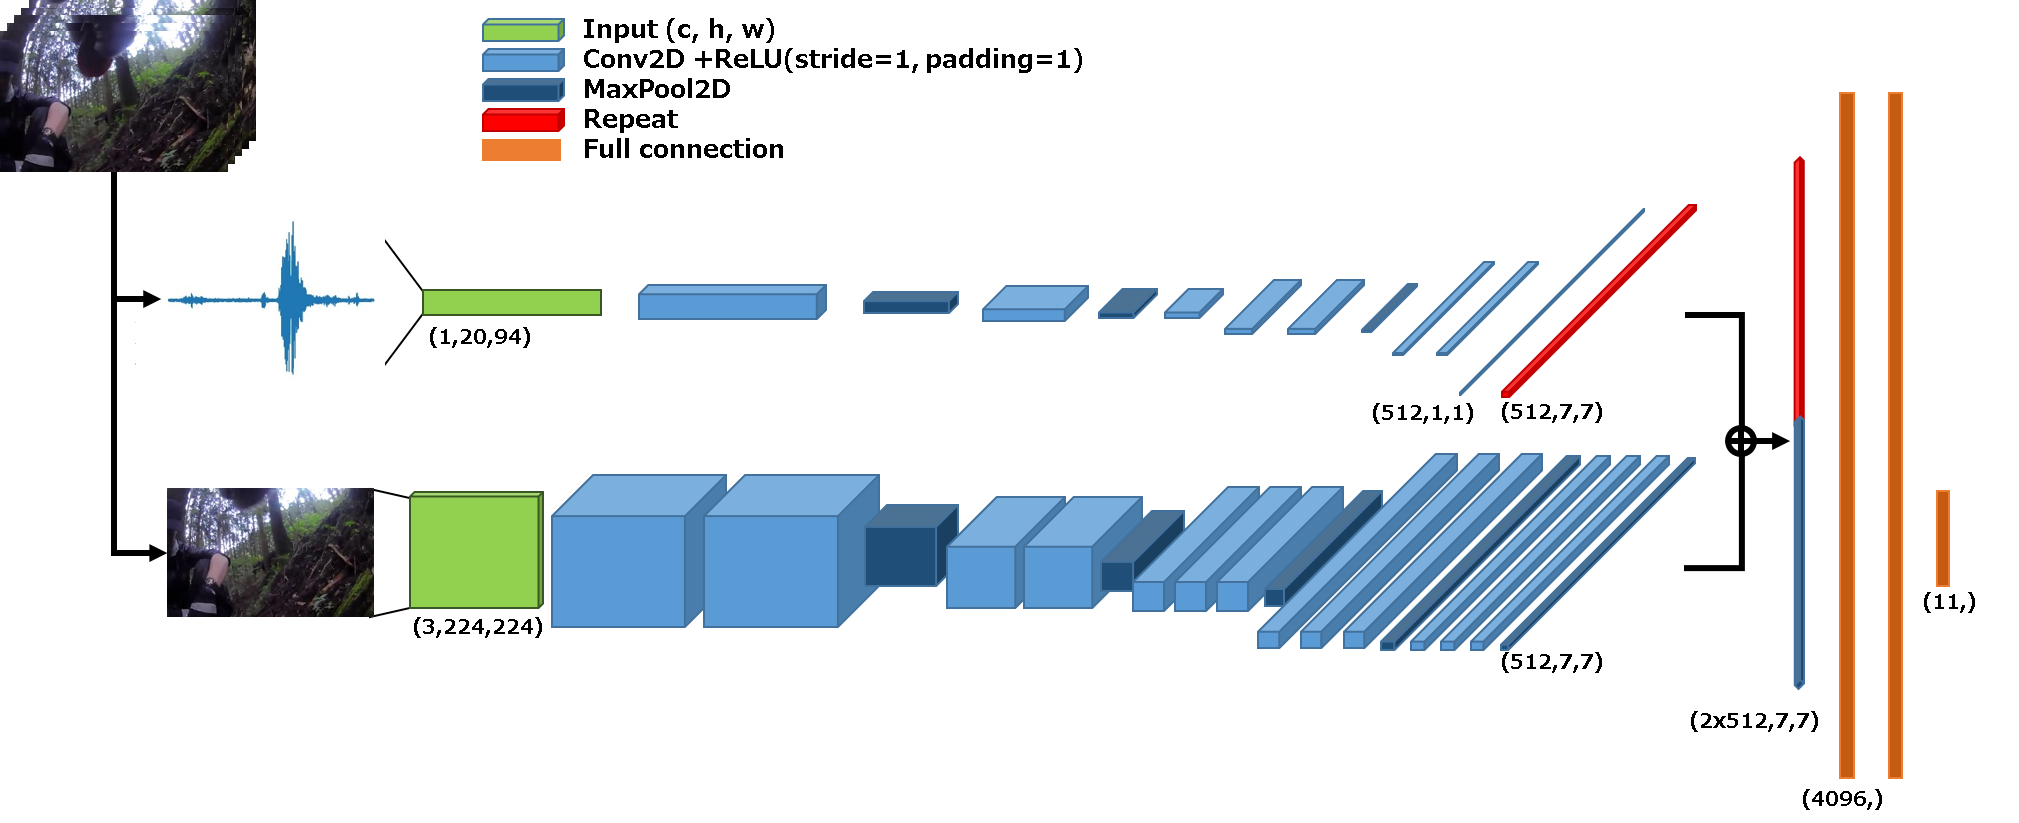
\includegraphics[width=15cm]{./Figures/soundbasedTwostream.eps}
  \caption{Sound/image-based two-stream CNN(提案手法)のアーキテクチャ.(3,224,224)次元の画像と(1,20,94)次元を音声をそれぞれ別のネットワークに通し,得られた特徴を結合したのちFCレイヤを通しクラス数と同じ次元の出力を得る.}
  \label{sound-two-stream}
 \end{center}
\end{figure}



\section{音声・静止画像・optical flow画像を用いたsound/image-based three-stream CNN}
2つ目の提案手法として,音声,静止画像,optical flow画像の3つの情報を用いたsound/image-based three-streamを提案する.
Sound/image-based two-stream networkに,画像を入力とするネットワークを加えた3つのstreamを組み合わせている.
Sound/image-based two-stream networkのアーキテクチャを図~\ref{sound-two-stream}に示す.
動画を31フレームとし,中央から切り出した静止画像とそれに対応する直後のoptical flow画像をそれぞれImageNetで学習済みのVGG16モデルに通し,畳み込み層の出力を結合する.
動画から切り出した音声は音声ストリームに入力する.畳み込みを繰り返すと特徴の縦横次元が小さくなるため,静止画像の畳み込みの出力と同じサイズになるように調整する.
調整は畳み込みで奥行き次元を揃えた後,同じ特徴をリピートし目的の大きさになるまでコピーして結合する.
本研究では入力音声は(1,20,94)次元の特徴に変換しており,畳み込みを繰り返して(512,1,1)次元にする.この細長い特徴を縦横に7つ並べ,(512,7,7)の特徴として静止画像とoptical flowの結合特徴に追加で結合する.

\begin{figure}[htbp]
 \begin{center}
  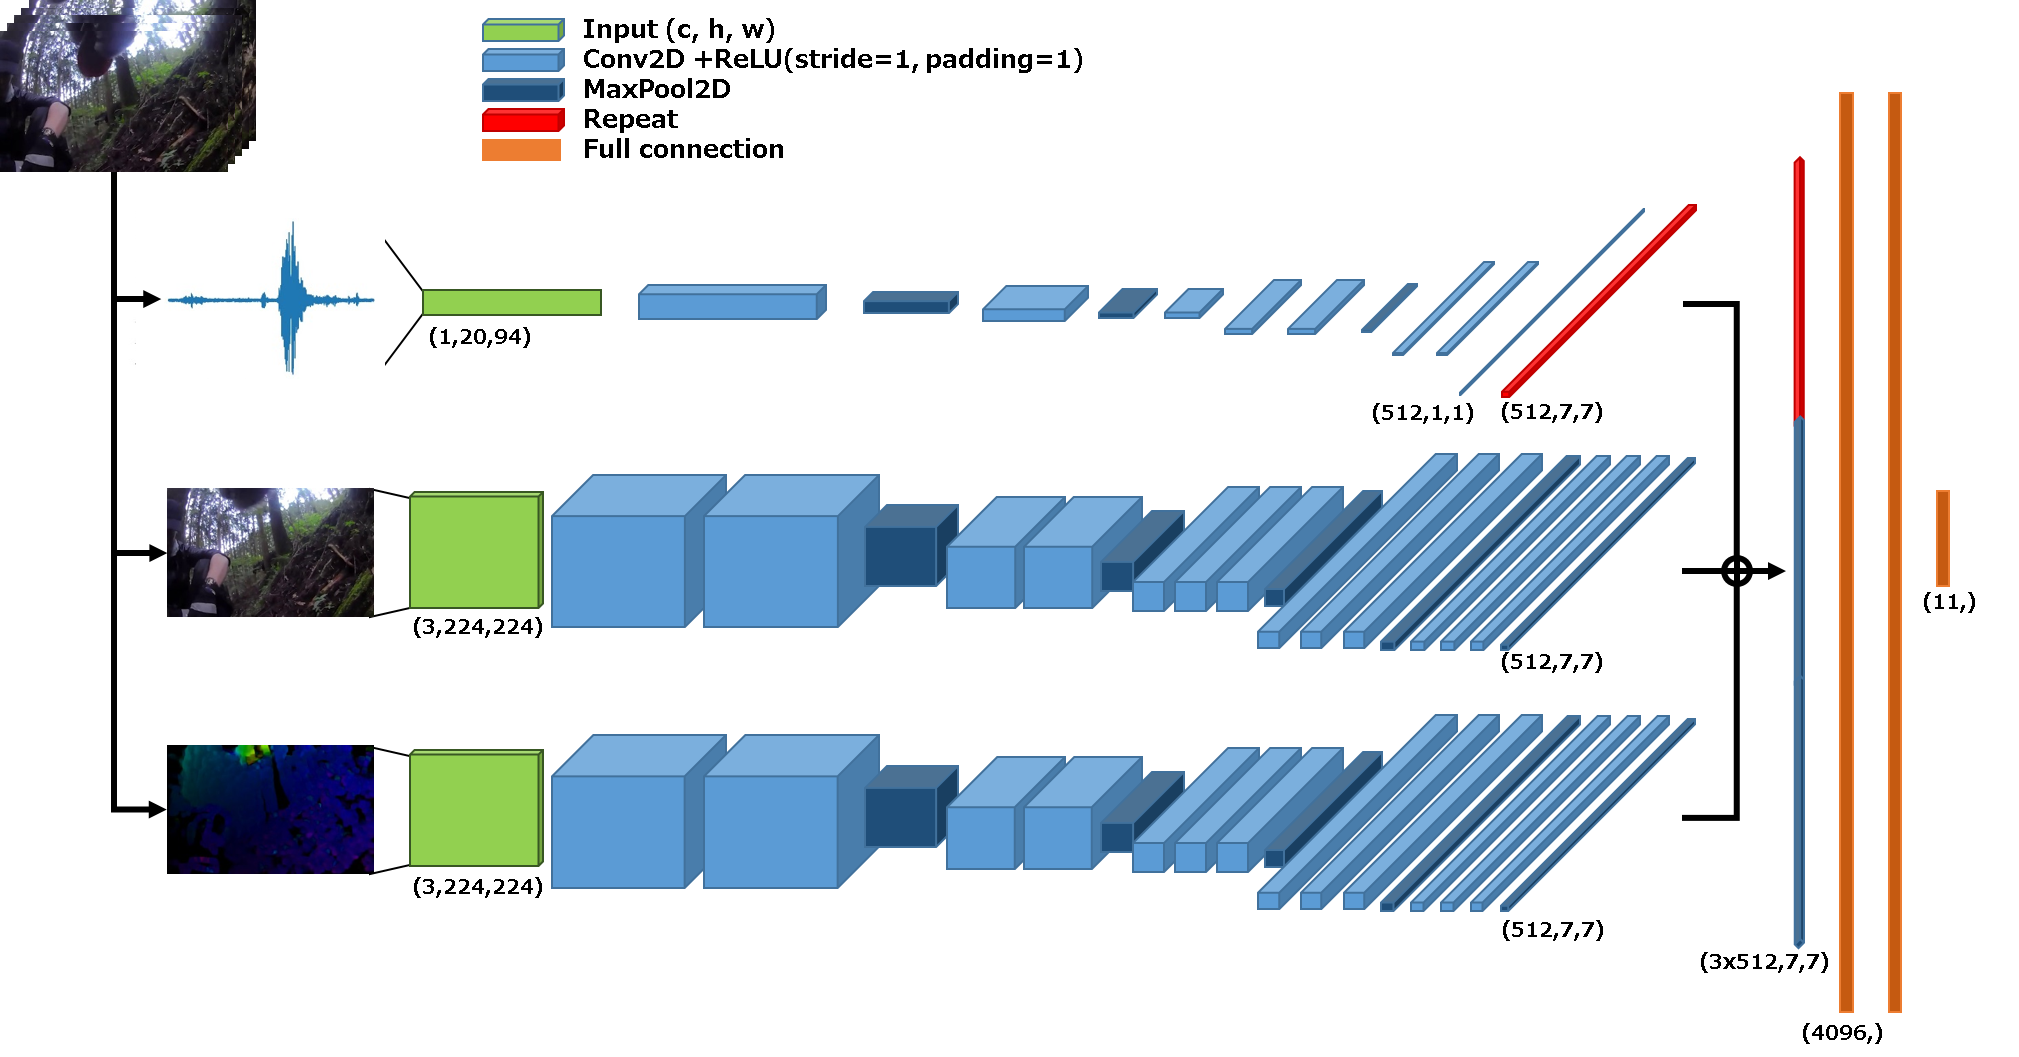
\includegraphics[width=15cm]{./Figures/soundbasedThreestream.eps}
  \caption{Sound/image-based three-stream CNN(提案手法)のアーキテクチャ.(3,224,224)次元の画像と(1,20,94)次元を音声をそれぞれ別のネットワークに通し,得られた特徴を結合したのちFCレイヤを通しクラス数と同じ次元の出力を得る.}
  \label{sound-three-stream}
 \end{center}
\end{figure}
